\section{Complexity analysis}\label{sec:complexity}

\subsection{Theoretical complexity}
The input-size parameters are the number of nodes $V$, the number of pipes $E$, the number of sources $|S|$ (2 in every instance), the number of locations to visit $n$ in T6 ($n=V$ for the full problem) and the number of candidate connections $n$ in T7. Table~\ref{tab:theory} gives the time and space cost of each implementation.

\begin{table}[H]
\centering\small
\caption{Theoretical complexity of the implementations. $m$: number of pipes reported by a range query; $h$: depth of the 2-d tree; $I$: number of hyper-heuristic iterations.}\label{tab:theory}
\begin{tabular}{llll}
\toprule
Task & Algorithm & Time & Space \\
\midrule
T1 & BFS, DFS, components on adjacency list & $O(V+E)$ & $O(V+E)$ \\
   & BFS, DFS, components on adjacency matrix & $O(V^2)$ & $O(V^2)$ \\
T2 & all pipe lengths & $O(E)$ & $O(E)$ \\
   & Floyd-Warshall (all pairs) & $O(V^3)$ & $O(V^2)$ \\
   & length query, linear scan & $O(E)$ & $O(E)$ \\
   & length query, hash index & $O(1)$ expected & $O(E)$ \\
   & sorting the lengths once & $O(E\log E)$ & $O(E)$ \\
   & range query on sorted lengths & $O(\log E+m)$ & $O(E)$ \\
T3 & repeated Dijkstra (binary heap) & $O(|S|(V+E)\log V)$ & $O(V+E)$ \\
   & multi-source Dijkstra & $O((V+E)\log V)$ & $O(V+E)$ \\
T4 & farthest node and route, given T3 & $O(V)$ & $O(V)$ \\
T5 & Edmonds-Karp & $O(VE^2)$ & $O(V+E)$ \\
   & Dinic & $O(V^2E)$ & $O(V+E)$ \\
T6 & metric closure (Floyd-Warshall) & $O(V^3)$ & $O(V^2)$ \\
   & nearest neighbour & $O(n^2)$ & $O(n)$ \\
   & one 2-opt pass & $O(n^2)$ & $O(n)$ \\
   & branch and bound, MST bound per node & $O(n!\,n^2)$ worst case & $O(n^2)$ \\
   & hyper-heuristic & $O(I\,n)$ & $O(n)$ \\
T7 & brute-force nearest node, per query & $O(n)$ & $O(n)$ \\
   & 2-d tree build & $O(n\log^2n)$ & $O(n)$ \\
   & 2-d tree query & $O(\log n)$ expected & $O(h)$ \\
   & 2-d tree insert & $O(h)$ & $O(1)$ \\
   & graph update, adjacency list & $O(1)$ amortised & $O(V+E)$ \\
   & graph update, adjacency matrix & $O(V^2)$ & $O(V^2)$ \\
\bottomrule
\end{tabular}
\end{table}

\subsection{Measurements}
Every time is the median of 21 samples, each sample repeating the call until it lasts at least 2\,ms so that timer resolution does not dominate; branch and bound uses the median of 3 runs because single runs take up to seconds. All measurements come from one machine (Python 3.13, Apple arm64). The four instances span only $20\le V\le71$, too narrow a range to show growth, so growth was measured on subsets of increasing size: induced PES sub-networks grown breadth-first from both sources ($V=10$ to 71) for T1 to T5, office-nearest subsets for T6 ($k=4$ to 16 locations) and random subsets of the PES candidates for T7 ($n=5$ to 69). Figure~\ref{fig:performance} compares each measured curve with its cost model scaled by a single fitted constant, and Table~\ref{tab:performance} gives the times on the four full instances. Absolute times include Python interpreter overhead, which dominates at these sizes; the relevant evidence is the growth rate and the ratio between alternatives.

\begin{figure}[H]
    \centering
    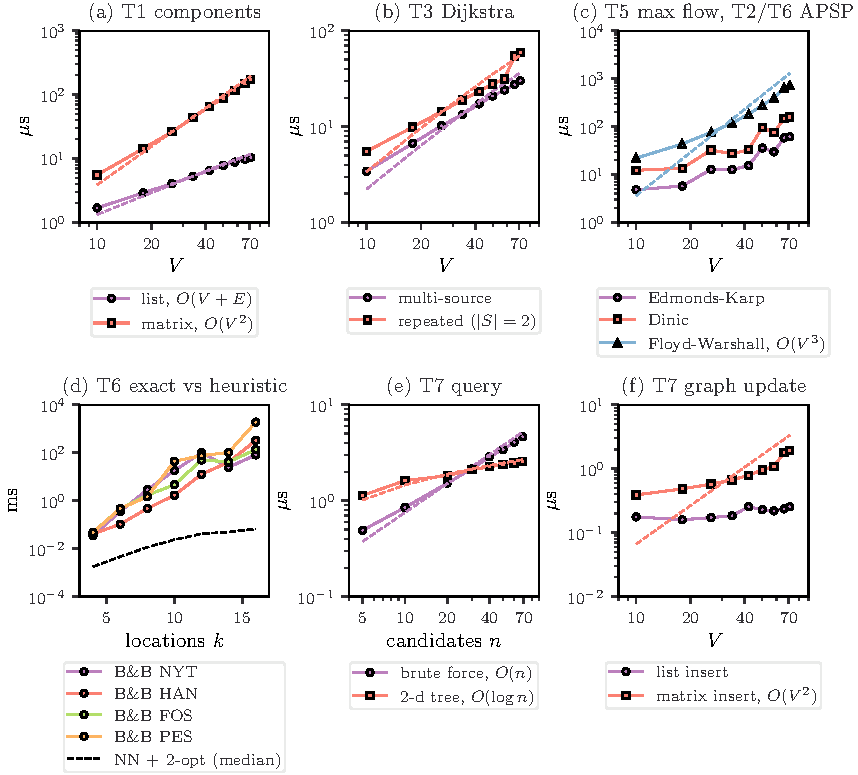
\includegraphics[width=\textwidth]{performance.pdf}
    \caption{Measured times (solid) against the theoretical cost model scaled to the data (dashed). All axes are logarithmic except the $k$ axis of (d), so that exponential growth in (d) appears as a straight line.}
    \label{fig:performance}
\end{figure}

\begin{table}[H]
\centering\footnotesize
\setlength{\tabcolsep}{4pt}
\caption{Median times in microseconds on the four instances; each column header gives the instance with $(V, E)$. Flow times cover both sectors; NN + 2-opt covers the full route; nearest-node times are for one query.}\label{tab:performance}
\begin{tabular}{lrrrr}
\toprule
\tablebody{performance}
\bottomrule
\end{tabular}
\end{table}

\subsection{Agreement with theory}
Most measurements follow their models. Component search grows with log-log slope about 0.9 on the adjacency list and 1.8 on the matrix (models 1 and 2), and the matrix is about 17 times slower at $V=71$, as $O(V^2)$ against $O(V+E)$ predicts for sparse graphs. Both Dijkstra variants follow $(V+E)\log V$, with slopes about 1.1 and 1.2. Repeated Dijkstra performs exactly twice the relaxations of the multi-source version and takes 1.4 times as long on the median subset and 2.0 times on the full PES network, where fixed overheads matter least.

Three measurements deviate from their models, each for an identifiable reason. The Floyd-Warshall time grows with slope about 1.8 instead of 3, because each of its $V$ steps is one vectorised NumPy update whose fixed cost dominates while the matrix has at most 5,041 cells; it still performs exactly $V^3$ elementary updates, and its curve steepens towards the $V^3$ reference as $V$ grows. Edmonds-Karp and Dinic grow far more slowly than $O(VE^2)$ and $O(V^2E)$ (Figure~\ref{fig:performance}c), because every source-sink pair needs at most four augmenting paths, each found by one $O(E)$ BFS; at this scale Edmonds-Karp is faster, about 2.5 times on the median sub-network and 1.6 to 2.2 times on the full instances, since Dinic's level graph and recursive blocking-flow search only pay off when a phase contains many augmenting paths. The matrix insertion grows about 5 times from $V=10$ to 71, much less than $V^2$, because copying a few thousand cells is cheap next to NumPy's allocation cost; the quadratic growth would dominate on larger networks.

Branch and bound is the only exponential cost. Its time multiplies by about 1.4 (NYT) to 2.2 (HAN) per added location, reaching about 2\,s at $k=16$ on PES, while NN + 2-opt stays below 0.1\,ms. The 2-d tree query grows logarithmically (3.5 to 11 distance evaluations) and beats brute force from about 30 candidates, but its build pays for itself only after a few tens of queries, so for the two or three insertions per instance brute force is sufficient.
